\chapter{Revisão Teórica} \label{revisão}
% [Futuramente, pode ser necessário expandir essa seção]

Esta seção visa oferecer os conceitos necessários para o completo entendimento desse trabalho. Inicialmente, serão apresentados os conceitos relacionados a classificação de satélites, os padrões CubeSat e PC104, alguns conceitos de eletrônica e, por fim, um histórico das missões anteriores

\section{Nanosatélites}
Normalmente, a classificação mais utilizada para satélites é com relação a sua massa. Na figura abaixo, podemos ver as categorias utilizadas nessa classificação e alguns exemplos de artefatos já lançados. Observe que os nanossatélites se encontram na faixa de 1 até 10 kg.

\noindent
\begin{minipage}{\linewidth}
\makebox[\linewidth]{
    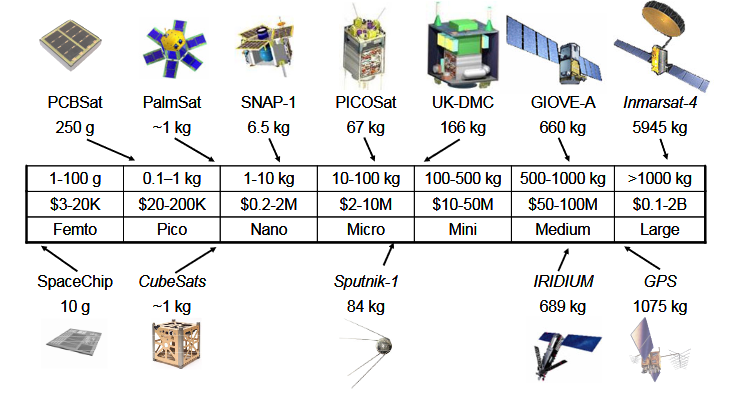
\includegraphics[keepaspectratio=true, scale=0.5]{imagens/Satellite-mass-classification.png}}
\label{mass_classification_fig}
\captionof{figure}{Classificação de satélites, com alguns exemplos}
\end{minipage}

 Os principais responsáveis por essa redução de massa são a miniaturização dos circuitos integrados e as padronizações das estruturas de lançamento, como no padrão \textit{Cubesat}. Os nanossatélites são amplamente utilizados nas atividades de ensino, pois permitem um ciclo completo de uma missão espacial mantendo um custo baixo, principalmente devido ao uso de peças comerciais.\cite{barnhart_ref}

\section{\textit{Cubesat}}\label{cubesat_specs}

O padrão \textit{Cubesat} foi um dos grandes responsáveis pela popularização da categoria de nanossatélites, como podemos ver no gráfico abaixo, que mostra o número de lançamentos desse tipo por ano.\cite{cubesats_cgee}.

\noindent
\begin{minipage}{\linewidth}
\makebox[\linewidth]{
    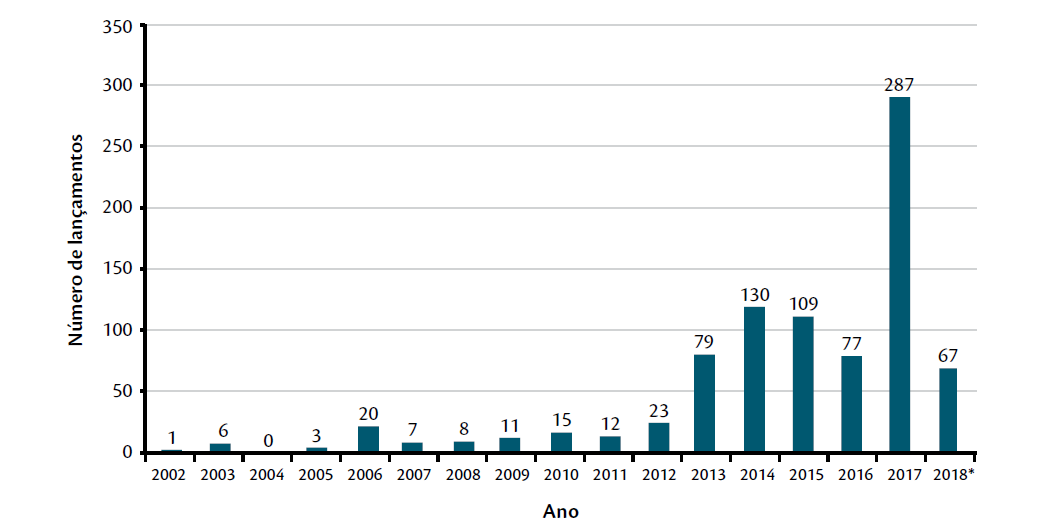
\includegraphics[keepaspectratio=true, scale=0.5]{imagens/cubesat-launches-count.png}}
\captionof{figure}{Distribuição do número de \textit{Cubesats} pelo ano de lançamento}
\label{cubesat_launches_fig}
\end{minipage}

O modelo \textit{Cubesat} foi proposto em 1999 por Jordi Puig-Suari, da \textit{California Polytechnic State University}, e Bob Twiggs, da \textit{Stanford University}. O objetivo era um modelo de satélite de pequeno porte que segue um padrão mais simples, o intuito deles era fornecer aos alunos de ambas universidades a oportunidade de  participar de um projeto espacial completo, incluindo todas as fases, desde a construção, testes e operação do artefato, que manteria características similares aos satélites maiores. 

O termo é um acrônimo entre as palavras \textit{cube} (em inglês, cubo) acrescida das três primeiras letras da palavra satélite.

Normalmente, as missões com \textit{Cubesats} tem um risco técnico mais elevado, em parte devido ao uso de componentes não \textit{"space qualified"}, porém oferecem em troca uma implementação mais rápida, aplicações mais inovadoras, custos menores ou um conjunto desses elementos.

As principais características dos \textit{Cubesats} são as seguintes:
\begin{itemize}
    \item compostos por unidades cúbicas padronizadas (1U) de tamanho 10x10x10 cm, conforme mostrado na figura \ref{cubesat_configs_fig};
    \item uso de sistemas padronizados de ejeção em órbita, denominados, P-POD (do inglês, \textit{Poly Picosatellite Orbital Deployer}) ou SSPL (do inglês, \textit{Space Shuttle Picosatellite Launcher}). Esses sistemas são capazes de liberar diversos satélites pela mesma interface;
    \item componentes COTS nos sistemas de bordo.
\end{itemize}

\noindent
\begin{minipage}{\linewidth}
\makebox[\linewidth]{
    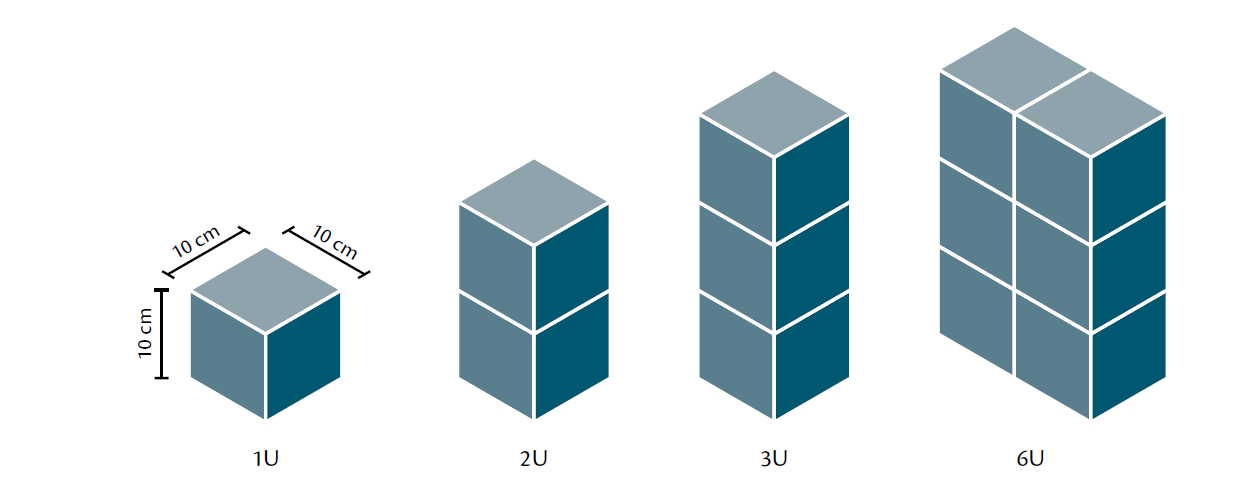
\includegraphics[keepaspectratio=true, scale=0.5]{imagens/cubesats-configs.png}}
\captionof{figure}{Algumas configurações de \textit{Cubesats}}
\label{cubesat_configs_fig}
\end{minipage}

O padrão é descrito em um documento de domínio público\cite{cubesat_specs_rev13}, onde especifica-se que uma unidade \textit{Cubesat} ou 1U, tem um volume de 1 litro e carga útil de até 1,3 kg, podendo combinar várias unidades dessas para compor satélites maiores (2U, 3U, 6U ou 12U, por exemplo).

\noindent
\begin{minipage}{\linewidth}
\makebox[\linewidth]{
    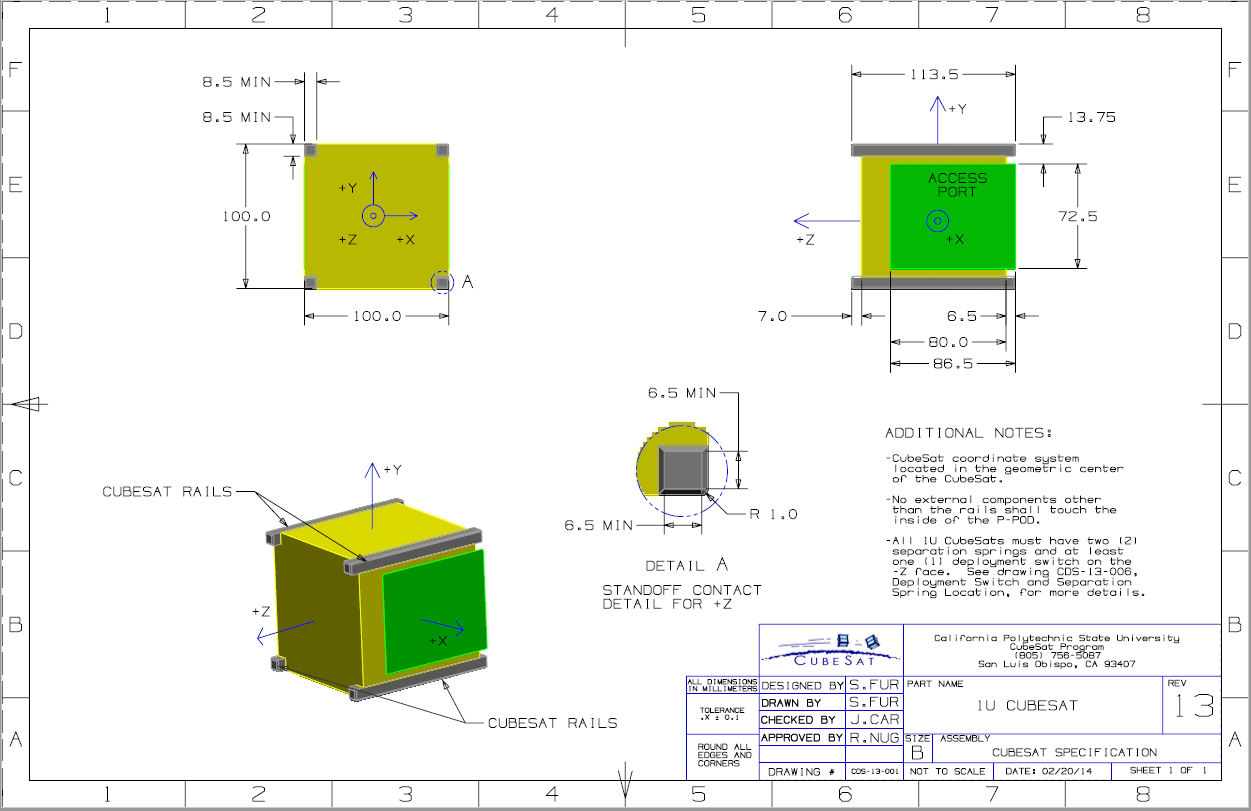
\includegraphics[keepaspectratio=true, scale=0.5]{imagens/Cubesat-diagram.png}}
\captionof{figure}{Especificações de dimensionamento para um \textit{Cubesat} 1U}
\label{cubesat1U_dimensions_fig}
\end{minipage}

Por esses e outros aspectos, os \textit{Cubesats} trouxeram um aspecto inovador capaz de mudar o paradigma do setor espacial, adequando-o à nova tendência de emprego de pequenos satélites para atender a diferentes tipos de demandas.

\section{Printed Circuit Board (PCB)}\label{pcb_revision}
\textit{Printed Circuit Board}, em português: placa de circuito impresso, é uma técnica amplamente utilizada na eletrônica que consiste em construir uma placa de um material isolante que apresenta em sua superfícies trilhas condutoras que representam o circuito em que serão soldados os dispositivos eletrônicos.

Para a maioria dos circuitos, ter apenas uma superficie condutora é insuficiente dado que algum momento durante o design será impossível evitar o cruzamento entre trilhas, portanto, a maioria das PCBs são multicamadas, ou seja, possuem múltiplas camadas de trilhas condutoras isoladas.

Essa forma de construir circuitos representou grande avanço na eletrônica, pois esse arranjo permite maior resistência a interferências, melhor fixação dos componentes e otimização no uso do espaço, possibilitando equipamentos menores.

O processo moderno de design de uma PCB é facilitado pelo uso de software de \textit{layout} dedicado que ao final do processo nos fornece os arquivos .gerber que serão usados para a fabricação, nesses arquivos não são colocadas informação sobre os componentes, há apenas as informações que o fabricante da PCB necessita, a exemplo das \textit{layers}, furações, entre outros.

\subsection{Ambiente espacial}
Um problema a ser considerado no desenvolvimento, especialmente das placas eletrônicas, é o efeito do ambiente espacial nos subsistemas. Os problemas causados podem variar desde mal funcionamento até danos físicos, normalmente essas considerações são feitas para missões de longa duração realizadas em \textit{LEO} (do inglês \textit{Low Space Orbit}) e \textit{Deep Space} \cite{nasa_state_of_art}.

A quantidade de radiação que incide nos satélites depende da altitude e do tipo da órbita. A maioria dos \textit{Cubesats} são colocados em órbitas LEO (entre 100 e 1000 km de altitude), recebendo uma dose de radiação de  aproximadamente 0,1 krad/ano.

A resistência a radiação é um dos grandes desafios das missões \textit{Cubesat}, pois os componentes COTS não tem nenhuma preocupação com radiação durante o processo de design, logo, os clientes desses componentes devem blindar todas as partes eletrônicas, realizar todos os testes de exposição e assumir os possíveis riscos de falhas.

\section{PC/104}\label{pc104_specs}
A rápida difusão do uso de computadores embarcados, especialmente em fins industriais, exigiu uma forma de ampliar recursos em plataforma SBC (do inglês, \textit{Single Board Computer}, computador de placa única), sem um grande custo ou espaço. Em fevereiro de 1992, foi criado o consórcio do padrão PC/104, que tinha por objetivo padronizar a tecnologia de computadores de bordo para aplicações embarcadas. O PC/104 se transformou no padrão para placas eletrônicas, um dos mais utilizados na indústria e em missões com Cubesats. Esse padrão definido pelo PC/104 \textit{Embedded Consortium} em 2008 e está disponível em documento de domínio público\cite{pc104_document}, nele são definidas restrições mecânicas e elétricas para uma PCB.

As restrições mais relevantes para a nossa aplicação seguem abaixo:

\begin{enumerate}
    \item A placa deve ter um formato de 90x96mm;
    \item A potência ativa do módulo deve estar entre 1-2W, limitando a corrente do barramento em 4\textit{m}A;
    \item Os módulos devem ser de 8 ou 16-bits, correspondentes aos barramentos PC e PC/AT, respectivamente;
    \item O espaçamento máximo entre as placas é de 15,24mm
    \item A altura máxima dos componentes na placa é de 11,05mm
    \item A utilização do barramento deve respeitar a tabela \ref{pc104_signal_assignments_table}
\end{enumerate}{}

A padronização PC/104 é ideal para missões Cubesat como o projeto Lodestar, pois as restrições de dimensões, barramentos, interfaces mecânicas e elétricas implicam em reduções no custo, riscos e tempo, na maioria das vezes. Sem contar o fato de ser um padrão amplamente utilizado, o que permite a integração de outros módulos que usem o mesmo padrão.

\noindent
\begin{minipage}{\linewidth}
\makebox[\linewidth]{
    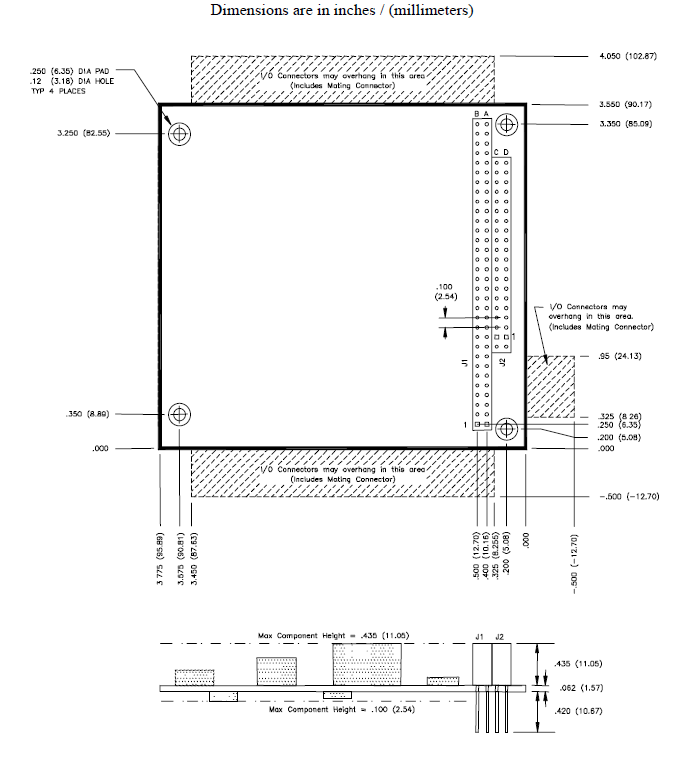
\includegraphics[keepaspectratio=true, scale=1]{imagens/PC104-dimensions.png}}
\captionof{figure}{Especificações de dimensionamento para um módulo de 16-bits PC/104}
\label{pc104_dimensions_fig}
\end{minipage}

\section{Microcontrolador/Microprocessador}\label{mcu_revision}

A principal diferenciação entre microcontroladores e microprocessadores está na quantidade de componentes que estão embarcados em um e outro. O microcontrolador (MCU) é um computador completo inteiro em um único circuito integrado, ou seja, contém memórias, timers, portas de comunicação serial, entre outros periféricos. Já o microprocessor contém essencialmente as unidades de controle e cálculo, necessitando de periféricos externos para formar um sistema minímo de um computador.

Os MCUs atualmente encontram uma enorme gama de aplicações na eletrônica moderna, desde máquinas industriais, sistemas embarcados a brinquedos e eletrodomésticos. São exemplos de microcontroladores: Texas Instruments MSP430, PIC, Atmel AVR, ARM Cortex-M, entre outros.

Para a nossa missão, a escolha do MCU é um ponto-chave, uma vez que ele é o componente mais importante do OBC, pois é o responsável por executar o \textit{software} destinado ao gerenciamento do satélite. Abaixo seguem alguns critérios importantes na escolha do MCU mais adequado:

\begin{enumerate}
    \item Baixo consumo: a disponibilidade de energia em órbia dependerá da área de cobertura e eficiência dos painéis solares e essa potência também será dividida com os outros subsistemas, logo, o nosso MCU tem que consumir pouco quando em funcionamento;
    \item Conversores AD: O OBC necessitará ler dados de muitos sensores, exemplo: temperatura e luminosidade;
    \item Portas I/O: As portas GPIO (do inglês \textit{General-Purpose Input/Output}) são essenciais para comunicação com os outros subsistemas;
    \item Interfaces Seriais: Ter pinos dedicados aos protocolos de comunicação serial (UART, I2C, SPI) ajudam no desenvolvimento do OBC;
    \item PWM: Para o controle de motores, consequentemente há necessidade de pinos que produzam PWM;
    \item Frequência de Operação: Deseja-se usar um microcontrolador com uma frequência de \textit{clock} elevada para ter uma melhor performance;
    \item Faixa de temperatura: O microcontrolador deve resistir a qualquer temperatura encontrada na órbita LEO.
\end{enumerate}

Mais adiante, no capítulo de desenvolvimento (\ref{desenvolvimento}) abordaremos a nossa escolha de microcontrolador e como esses e outros critérios foram avaliados.


\section{Histórico de missões anteriores}\label{missions_history}

Um levantamento de trabalho com escopo semelhante a este foi realizado e a Tabela \ref{history_table} mostra alguns exemplos de \textit{CubeSats}, indicando a missão, o tamanho, ano de deploy e quais as soluções utilizadas.

\begin{table}
\centering
\caption{Missões anteriores com \textit{Cubesats}}
\label{history_table}
\begin{tabular}{|l|l|l|l|} 
\hline
\multicolumn{1}{|c|}{Nome} & \multicolumn{1}{c|}{Tipo} & \multicolumn{1}{c|}{Ano} & \multicolumn{1}{c|}{Implementação do EPS}  \\ 
\hline
Cute 1.7+                  & Demonstração              & 2008                     &  Implementação do MPPT, centralizado  \\ 
\hline
SNAP-1                     & Demonstração              & 2000                     &  Implementação do MPPT, parcialmente distribuído  \\
\hline
ESTCube-1                  & Científico                & 2013                     &  Controladores MPPT, centralizado     \\ 
\hline
SwissCube                  & Observação                & 2009                     &  Implementação do MPPT, centralizado  \\
\hline
\end{tabular}
\end{table}

O CUTE \cite{cute1_ref} (Cubical  Tóquio  Tech  Engineering  Satellite-I) é um projeto cooperativo do LSS (Laboratory for Space Systems) e o SRTL (Space Robotics and Teleoperations Laboratory), ambos de Tóquio. O computador de bordo foi implementado com um processador Hitachi NPD-20JWL e executava o sistema operacional Windows CE.NET. O  projeto  educacional  de  baixo  custo  usava componentes COTS para uma missão de demonstração tecnológica, o projeto teve diversões lançamentos (Cute-I, Cute 1.7+ APD, Cute 1.7+ APD II). 

O SNAP-1 \cite{snap1_ref} foi o primeiro nanossatélite desenvolvido no Reino Unido pela Surrey Space Centre (SSC) e Surrey Satellite Tecnology Ltd (SSTL) e serviu como veículo de teste para demonstração da nova tecnologia que estava surgindo, ele foi um dos pioneiros dessa nova filósofia de design e mostrou que era possível construir um nanossatélite rapidamente e com custo baixo, utilizando peças COTS.

SamSat-218D \cite{samsat218_ref} foi um nanossatélite desenvolvido na \textit{Samara State Aerospace University}, lançado em 2015, e foi criado com o objetivo de ser uma plataforma de testes para tecnologias de navegação e controle. Além disso, o projeto foi utilizado para testar um OBC experimental, que empregava os processadores ATXmega 128U4 e LPC4357 DualCore, testar o controle de voo em condições anormais e novos painéis solares.

ESTCube-1 \cite{estcube1_ref} foi um \textit{cubesat} 1U lançado pelo foguete Vega VV02. Desenvolvido por uma força tarefa de 4 universidades, tinha o objetivo científico de realizar um prova de conceito de medição e demonstração da tecnologia da tecnologia de velas solares elétricas. Para o OBC um STMicroelectronics STM32F103 (ARM 32bits) foi escolhido para fazer os cálculos.

Cat-2 \cite{cat2_ref} foi um projeto de \textit{cubesat} 6U desenvolvido na \textit{Universitat Politècnica de Catalunya} e iniciado em 2009 para lançar um nanossatélite plataforma para um instrumento GNSS-R (do inglês, \textit{Global Navigation Satellite Systems Reflectometry}) que realizaria altimetria oceânica. A computação de bordo ficou a cargo de um ARM7TDMI.  

O SwissCube-1, \cite{swisscube_ref} foi um \textit{cubesat} suíço científico de tamanho 1U, operado pela Ecole Polytechnique Fédérale de Lausanne (EPFL) para realizar pesquisas sobre o \textit{nightglow} (fenômeno de brilho   noturno na atmosfera terrestre) e também para desenvolver tecnologia para futuras naves espaciais. A  computação  de  bordo utilizava um processador ARM7TDMI e o sistema operacional de tempo real FreeRTOS.

% Segundo \cite{soares2007ginga}:

% \begin{quote}
% 	Lorem ipsum dolor sit amet, consectetuer adipiscing elit. Ut purus elit, vesti- bulum ut, placerat ac, adipiscing vitae, felis. Curabitur dictum gravida mauris. Nam arcu libero, nonummy eget, consectetuer id, vulputate a, magna. 
% \end{quote}

% \lstset{caption=Exemplo de aplicação servidora, label=list:server}
% \begin{lstlisting}[language=C]
% int main()
% { 
%     FILE *fp;     int len;     
%     static const int SIZE = 1024;
%     struct sockaddr_in me, target;
%     int sock=socket(AF_INET,SOCK_DGRAM,0);
%     char arquivo[SIZE];
%     me.sin_family=AF_INET;
%     me.sin_addr.s_addr=htonl(INADDR_ANY); // endereco IP local 
%     me.sin_port=htons(0); // porta local (0=auto assign)
%     bind(sock,(struct sockaddr *)&me,sizeof(me));
%     target.sin_family=AF_INET;
%     target.sin_addr.s_addr=inet_addr("192.168.68.217"); // host local 
%     target.sin_port=htons(8450); // porta de destino 

%     if ((fp = fopen("video1.mp4","rb")) == NULL){
%         printf("Arquivo nao pode ser aberto.\n"); return -1;
%     }

%     while(!feof(fp)) {
%         len = fread(arquivo, 1, sizeof(arquivo), fp);
%         sendto(sock,arquivo,sizeof(arquivo),0,(struct sockaddr *)&target,sizeof(target));
%     }
%     sendto(sock,"FIM",sizeof("FIM"),0,(struct sockaddr *)&target,sizeof(target));
%     close(sock);
%     return 0;
% }
% \end{lstlisting}
